%%%%%%%%%%%%%%%%%%%%%%%%%%%%%%%%%%%%%%%%%%%%%%%%%%%%%%%%%%%%%%%%%%%%%%%%%%%%%%%%
%% Plantilla de memoria en LaTeX para la ETSIT - Universidad Rey Juan Carlos
%%
%% Por Gregorio Robles <grex arroba gsyc.urjc.es>
%%     Grupo de Sistemas y Comunicaciones
%%     Escuela Técnica Superior de Ingenieros de Telecomunicación
%%     Universidad Rey Juan Carlos
%% (muchas ideas tomadas de Internet, colegas del GSyC, antiguos alumnos...
%%  etc. Muchas gracias a todos)
%%
%% La última versión de esta plantilla está siempre disponible en:
%%     https://github.com/gregoriorobles/plantilla-memoria
%%
%% Para obtener PDF, ejecuta en la shell:
%%   make
%% (las imágenes deben ir en PNG o JPG)

%%%%%%%%%%%%%%%%%%%%%%%%%%%%%%%%%%%%%%%%%%%%%%%%%%%%%%%%%%%%%%%%%%%%%%%%%%%%%%%%

\documentclass[a4paper, 12pt]{book}
%\usepackage[T1]{fontenc}

\usepackage[a4paper, left=2.5cm, right=2.5cm, top=3cm, bottom=3cm]{geometry}
\usepackage{times}
\usepackage[utf8]{inputenc}
\usepackage[spanish]{babel} % Comenta esta línea si tu memoria es en inglés
\usepackage{url}
%\usepackage[dvipdfm]{graphicx}
\usepackage{graphicx}
\usepackage{float}  %% H para posicionar figuras
\usepackage[nottoc, notlot, notlof, notindex]{tocbibind} %% Opciones de índice
\usepackage{latexsym}  %% Logo LaTeX

\title{Memoria del Proyecto}
\author{Iván Miguel Molinero}

\renewcommand{\baselinestretch}{1.5}  %% Interlineado

\begin{document}

\renewcommand{\refname}{Bibliografía}  %% Renombrando
\renewcommand{\appendixname}{Apéndice}

%%%%%%%%%%%%%%%%%%%%%%%%%%%%%%%%%%%%%%%%%%%%%%%%%%%%%%%%%%%%%%%%%%%%%%%%%%%%%%%%
% PORTADA

\begin{titlepage}
\begin{center}
\includegraphics[scale=0.8]{img/URJ_logo_Color_POS.png}

\vspace{1.75cm}

\Large
GRADO EN INGENIERÍA EN SISTEMAS AUDIOVISUALES
Y MULTIMEDIA

\vspace{0.4cm}

\large
Curso Académico 2022/2023

\vspace{0.8cm}

Trabajo Fin de Grado

\vspace{2.5cm}

\LARGE
EVALUACIÓN SISTEMÁTICA DE PROYECTOS DE SOFTWARE LIBRE

\vspace{4cm}

\large
Autor : Iván Miguel Molinero \\
Tutor : Dr. Gregorio Robles Martínez
\end{center}
\end{titlepage}

\newpage
\mbox{}
\thispagestyle{empty} % para que no se numere esta pagina


%%%%%%%%%%%%%%%%%%%%%%%%%%%%%%%%%%%%%%%%%%%%%%%%%%%%%%%%%%%%%%%%%%%%%%%%%%%%%%%%
%%%% Para firmar
\clearpage
\pagenumbering{gobble}
\chapter*{}

\vspace{-4cm}
\begin{center}
\LARGE
\textbf{Trabajo Fin de Grado/Máster}

\vspace{1cm}
\large
Evaluación Sistemática de Proyectos de Software Libre

\vspace{1cm}
\large
\textbf{Autor :} Iván Miguel Molinero \\
\textbf{Tutor :} Dr. Gregorio Robles Martínez

\end{center}

\vspace{1cm}
La defensa del presente Proyecto Fin de Carrera se realizó el día \qquad$\;\,$ de \qquad\qquad\qquad\qquad \newline de 202X, siendo calificada por el siguiente tribunal:


\vspace{0.5cm}
\textbf{Presidente:}

\vspace{1.2cm}
\textbf{Secretario:}

\vspace{1.2cm}
\textbf{Vocal:}


\vspace{1.2cm}
y habiendo obtenido la siguiente calificación:

\vspace{1cm}
\textbf{Calificación:}


\vspace{1cm}
\begin{flushright}
Fuenlabrada, a \qquad$\;\,$ de \qquad\qquad\qquad\qquad de 202X
\end{flushright}

%%%%%%%%%%%%%%%%%%%%%%%%%%%%%%%%%%%%%%%%%%%%%%%%%%%%%%%%%%%%%%%%%%%%%%%%%%%%%%%%
%%%% Dedicatoria

\chapter*{}
\pagenumbering{Roman} % para comenzar la numeracion de paginas en numeros romanos
\begin{flushright}
\textit{Hazlo o no lo hagas, \\
pero no lo intentes. \\
Maestro Yoda}
\end{flushright}

%%%%%%%%%%%%%%%%%%%%%%%%%%%%%%%%%%%%%%%%%%%%%%%%%%%%%%%%%%%%%%%%%%%%%%%%%%%%%%%%
%%%% Agradecimientos

\chapter*{Agradecimientos}
%\addcontentsline{toc}{chapter}{Agradecimientos} % si queremos que aparezca en el índice
\markboth{AGRADECIMIENTOS}{AGRADECIMIENTOS} % encabezado 

Aquí vienen los agradecimientos\ldots Aunque está bien acordarse de la pareja, no hay que olvidarse de dar las gracias a tu madre, que aunque a veces no lo parezca disfrutará tanto de tus logros como tú\ldots 
Además, la pareja quizás no sea para siempre, pero tu madre sí.

%%%%%%%%%%%%%%%%%%%%%%%%%%%%%%%%%%%%%%%%%%%%%%%%%%%%%%%%%%%%%%%%%%%%%%%%%%%%%%%%
%%%% Resumen

\chapter*{Resumen}
%\addcontentsline{toc}{chapter}{Resumen} % si queremos que aparezca en el índice
\markboth{RESUMEN}{RESUMEN} % encabezado

Aquí viene un resumen del proyecto.
Ha de constar de tres o cuatro párrafos, donde se presente de manera clara y concisa de qué va el proyecto. 
Han de quedar respondidas las siguientes preguntas:

\begin{itemize}
  \item ¿De qué va este proyecto? ¿Cuál es su objetivo principal?
  \item ¿Cómo se ha realizado? ¿Qué tecnologías están involucradas?
  \item ¿En qué contexto se ha realizado el proyecto? ¿Es un proyecto dentro de un marco general?
\end{itemize}

Lo mejor es escribir el resumen al final.

%%%%%%%%%%%%%%%%%%%%%%%%%%%%%%%%%%%%%%%%%%%%%%%%%%%%%%%%%%%%%%%%%%%%%%%%%%%%%%%%
%%%% Resumen en inglés

\chapter*{Summary}
%\addcontentsline{toc}{chapter}{Summary} % si queremos que aparezca en el índice
\markboth{SUMMARY}{SUMMARY} % encabezado

Here comes a translation of the ``Resumen'' into English. 
Please, double check it for correct grammar and spelling.
As it is the translation of the ``Resumen'', which is supposed to be written at the end, this as well should be filled out just before submitting.


%%%%%%%%%%%%%%%%%%%%%%%%%%%%%%%%%%%%%%%%%%%%%%%%%%%%%%%%%%%%%%%%%%%%%%%%%%%%%%%%
%%%%%%%%%%%%%%%%%%%%%%%%%%%%%%%%%%%%%%%%%%%%%%%%%%%%%%%%%%%%%%%%%%%%%%%%%%%%%%%%
% ÍNDICES %
%%%%%%%%%%%%%%%%%%%%%%%%%%%%%%%%%%%%%%%%%%%%%%%%%%%%%%%%%%%%%%%%%%%%%%%%%%%%%%%%

% Las buenas noticias es que los índices se generan automáticamente.
% Lo único que tienes que hacer es elegir cuáles quieren que se generen,
% y comentar/descomentar esa instrucción de LaTeX.

%%%% Índice de contenidos
\tableofcontents 
%%%% Índice de figuras
\cleardoublepage
%\addcontentsline{toc}{chapter}{Lista de figuras} % para que aparezca en el indice de contenidos
\listoffigures % indice de figuras
%%%% Índice de tablas
%\cleardoublepage
%\addcontentsline{toc}{chapter}{Lista de tablas} % para que aparezca en el indice de contenidos
%\listoftables % indice de tablas


%%%%%%%%%%%%%%%%%%%%%%%%%%%%%%%%%%%%%%%%%%%%%%%%%%%%%%%%%%%%%%%%%%%%%%%%%%%%%%%%
%%%%%%%%%%%%%%%%%%%%%%%%%%%%%%%%%%%%%%%%%%%%%%%%%%%%%%%%%%%%%%%%%%%%%%%%%%%%%%%%
% INTRODUCCIÓN %
%%%%%%%%%%%%%%%%%%%%%%%%%%%%%%%%%%%%%%%%%%%%%%%%%%%%%%%%%%%%%%%%%%%%%%%%%%%%%%%%

\cleardoublepage
\chapter{Introducción}
\label{chap:introducción}
\label{sec:intro} % etiqueta para poder referenciar luego en el texto con ~\ref{sec:intro}
\pagenumbering{arabic} % para empezar la numeración de página con números

Actualmente se comparten muchos proyectos de software libre en Internet en general y en Github~\cite{website:GitHub}\footnote{\url{https://github.com/}} en particular. Algunos ejemplos de proyectos que se comparten son paquetes de Python que
ayudan a desarrolladores a no tener que "reinventar la rueda", es decir, que si necesitas hacer un proyecto que lea URLs en uno de sus pasos (por ejemplo) y alguien ya ha hecho un paquete para
ello, debes usar ese paquete para poder avanzar en tu proyecto de una forma más rápida y eficaz.

Un proyecto de software libre es un desarrollo que es público; los demás desarrolladores pueden verlo y mejorarlo a través de Pull Request y también descargarlo gratuitamente para su uso por eso muchos usuarios lo prefieren a proyectos de código cerrado.

Ahora bien, en Github se comparten infinidad de proyectos de software libre y no siempre es fácil distinguir entre los que son buenos y los que no lo son tanto: ¿cuál es más seguro? o ¿cuál es más eficiente?
Para resolver estas y más preguntas es que, gracias al paquete PyGithub\footnote{\url{https://github.com/pygithub/pygithub}}, he desarrollado esta aplicación web que permite al usuario introducir el nombre de un repositorio y analizarlo según los parámetros que más
le convengan.

El proyecto\cite{website:RepositorioTFG}  nace como una extensión de OpenBRR\footnote{\url{https://link.springer.com/chapter/10.1007/978-3-642-13244-5_18}} que es una forma de analizar proyectos en función a los siguientes 6 parámetros: funcionalidad, calidad, soporte, comunidad, adopción y usabilidad.
A estos parámetros se les asigna un peso y a partir de ahí, da una calificación final sobre 5 del proyecto. A parte de OpenBRR existen otras formas de analizar proyectos como OSMM, OpenBQR o MOSST entre muchos otros pero me decanté por esta opción al ser la que más se 
centraba en analizar los proyectos de software libre.

Esta herramienta ayudará a docentes y desarrolladores a distinguir entre los miles de repositorios de Github cuáles son los que merecen la pena agilizando mucho la búsqueda. Pongamos un ejemplo práctico para que se entienda mejor: un desarrollador busca un paquete
que realice una función específica para su proyecto pero si tiene que buscar entre las miles de opciones cuál es la mejor, tardaría un tiempo excesivo ya que tendría que analizar cada código por si mismo (con todo lo que ello supone como entenderlo si no está bien comentado),
buscar vulnerabilidades, descargarlo, probarlo , etc. En cambio, gracias a este proyecto podrá buscar su mejor opción configurando el análisis según le convenga pudiendo poner el foco solo en seguridad, en seguridad y funcionalidad o en los 6 apartados que tiene OpenBRR.


\section{Estructura de la memoria}
\label{sec:estructura}

\begin{itemize}
  \item Capítulo~\ref{chap:introducción}: se explica brevemente el origen del proyecto, sus bases y funcionamiento .
  
  \item Capítulo~\ref{chap:objetivos}: se muestran los objetivos del proyecto.
  
  \item A continuación se presenta el estado del arte en el capítulo~\ref{chap:estado}.
  
  \item \ldots
\end{itemize}



%%%%%%%%%%%%%%%%%%%%%%%%%%%%%%%%%%%%%%%%%%%%%%%%%%%%%%%%%%%%%%%%%%%%%%%%%%%%%%%%
%%%%%%%%%%%%%%%%%%%%%%%%%%%%%%%%%%%%%%%%%%%%%%%%%%%%%%%%%%%%%%%%%%%%%%%%%%%%%%%%
% OBJETIVOS %
%%%%%%%%%%%%%%%%%%%%%%%%%%%%%%%%%%%%%%%%%%%%%%%%%%%%%%%%%%%%%%%%%%%%%%%%%%%%%%%%

\cleardoublepage % empezamos en página impar
\chapter{Objetivos} % título del capítulo (se muestra)
\label{chap:objetivos} % identificador del capítulo (no se muestra, es para poder referenciarlo)

\section{Objetivo general} % título de sección (se muestra)
\label{sec:objetivo-general} % identificador de sección (no se muestra, es para poder referenciarla)

Mi trabajo de fin de grado consiste en crear una aplicación web que analice repositorios de Github para darles una calificación sobre 5 basándose en los parámetros de OpenBRR.


\section{Objetivos específicos}
\label{sec:objetivos-especificos}

A la hora de realizar este proyecto, he abordado los siguientes objetivos específicos:

\begin{itemize}
	\item Estudiar, aprender y utilizar Django\footnote{\url{https://www.djangoproject.com/}}.

	\item Estudiar qué es OpenBRR y saber cómo analizar un código para poder calificar cada uno de sus parámetros.
	
	\item Analizar el paquete PyGithub en busca de las funciones que necesitaba para analizar repositorios.

	\item Rellenar y enviar formularios con Django.

	\item Manipular los datos enviados por el usuario y enviar los resultados.

	\item Probar el proyecto tanto con repositorios vacíos, como con repositorios teóricamente buenos para comprobar si los resultados eran coherentes.

	\item Solucionar errores como que el usuario introduzca un repositorio que no exista.

	\item Introducir mejoras tales como permitir al usuario introducir una dirección de correo electrónico para que le lleguen los resultados ahí también.

	\item Probar aún más repositorios haciendo que la aplicación se centrase en diferentes parámetros para comprobar que hacía un correcto análisis.
\end{itemize}


\section{Planificación temporal}
\label{sec:planificacion-temporal}

El proyecto se empezó a pensar a finales de Febrero de 2022 pero no fue hasta el verano de ese año que se empezó a trabajar en serio en él ya que anteriormente tenía que compaginarlo con las prácticas externas y no disponía del tiempo necesario. 
De Marzo a Junio de 2022 dedicaba las mañanas de los sábados y domingos a investigar qué era OpenBRR, en qué consistía y cómo podía usarlo para este proyecto. Asimismo mi tutor me recomendó usar el paquete Perceval\footnote{\url{https://perceval.readthedocs.io/en/latest/perceval/git.html}} de Python para analizar los repositorios de GitHub pero tras investigar por mi cuenta di con el paquete PyGithub el cual analizaba los repositorios de una forma más rápida y cómoda para el desarrollador ya que únicamente con introducir el nombre del repositorio es capaz de sacar todos los datos necesarios.

Durante el verano, pasaba las mañanas de lunes a viernes trabajando en el TFG y conseguí entender el funcionamiento completo de PyGithub así como analizar todos los datos que me devolvía y relacionarlos con los 6 parámetros de OpenBRR intentando que cada dato perteneciera al parámetro que más le correspondiera.

En el mes de Septiembre decidí implementar Django en la aplicación para ser capaz de leer, manipular y crear páginas web a través de las peticiones del usuario. No tenía conocimientos sobre esta tecnología así que usé los tutoriales de DjangoGirls\footnote{\url{https://djangogirls.org/es/}}\cite{website:DjangoGirls} para aprender a utilizarla dedicando 3 tardes de lunes a viernes y las mañanas de los sábados y domingos.

Finalmente, de Octubre de 2022 a Enero de 2023, empecé con el desarrollo de la aplicación web dedicando el mismo reparto de tiempo que para aprender Django ya que tenía clases de la universidad por las mañanas salvo en las vacaciones de Navidad que le dediqué todas las mañanas sin excepción. Durante el desarrollo surgieron varias dudas como qué datos asignar a qué parámetros y, sobretodo, qué peso asignarle a cada dato pero tras varias reuniones con mi tutor decidimos que el usuario pudiera manejar los pesos a su antojo para así poder centrarse en analizar los repositorios de la forma que más le convenga.
A finales de Diciembre comencé a hacer pruebas con repositorios profesionales como el propio de PyGithub o los de myTeachingURJC\footnote{\url{https://github.com/myTeachingURJC}} (los cuales son utilizados por los profesores de la universidad para compartir contenido de sus asignaturas) y con repositorios de peor calidad como mis primeros repositorios en busca de evaluaciones coherentes y algún error. Para principios de Enero la aplicación ya era funcional pero no tenía ningún tipo de estilo así que dediqué el resto del tiempo a personalizar su aspecto, así como a corregir y controlar errores que surgían durante las diferentes pruebas que realizaba.
Por tanto, dediqué las mañanas de finales de Enero y todo Febrero para la realización de la memoria con el objetivo de poder presentar el proyecto en Marzo.

%%%%%%%%%%%%%%%%%%%%%%%%%%%%%%%%%%%%%%%%%%%%%%%%%%%%%%%%%%%%%%%%%%%%%%%%%%%%%%%%
%%%%%%%%%%%%%%%%%%%%%%%%%%%%%%%%%%%%%%%%%%%%%%%%%%%%%%%%%%%%%%%%%%%%%%%%%%%%%%%%
% ESTADO DEL ARTE %
%%%%%%%%%%%%%%%%%%%%%%%%%%%%%%%%%%%%%%%%%%%%%%%%%%%%%%%%%%%%%%%%%%%%%%%%%%%%%%%%

\cleardoublepage
\chapter{Estado del arte}
\label{chap:estado}

Para la realización de este proyecto se ha utilizado Python, PyGithub, Github, Django, HTML, CSS, Javascript y OpenBRR.

\section{Python}
\label{sec:python}

Python\cite{website:Python} es un lenguaje de programación interpretado que le da importancia a la legibilidad del código teniendo una sintaxis muy limpia. Está orientado a objetos y permite ser un buen lenguaje para aprender a programar ya que tiene una curva de aprendizaje muy suave qracias a su sintaxis muy cercana al lenguaje humano. En un lenguaje de código abierto, lo que le permite estar en constante mejora por parte de los usuarios y ser adaptado para diferentes usos como el Machine Learning.

Python fue creado por Guido van Rossum en 1991 mientras trabajaba en el sistema operativo Amoeba\footnote{\url{https://www.cs.vu.nl/pub/amoeba/}} teniendo como objetivo controlar excepciones y manejar interfaces de dicho sistema operativo. A finales del año 2000 nació Python 2.0 el cual soportaba Unicode por primera vez y empezó a ser desarrollado por la comunidad bajo la mirada de Guido. Finalmente, en 2008 se lanzó Python 3.0 siendo la versión más completa de Python pero incompatible con las anteriores por lo que muchas características se implementaron también en Python 2.6.

La filosofía de Python se basa en los siguientes puntos para hacer la vida más fácil al desarrollador:

 \begin{itemize}
 	\item Hermoso es mejor que feo.
	\item Explícito es mejor que implícito.
 	\item Simple es mejor que complejo.
 	\item Plano es mejor que anidado.
 	\item Disperso es mejor que denso.
 	\item El código legible cuenta.
	\item Casos especiales no son lo suficientemente 	especiales para romper las reglas.
	\item Casi siempre lo práctico vence a lo formal
	\item Los errores no deben pasar nunca desapercibidos, a menos que se
especifique este comportamiento.
	\item Ante una ambigüedad, descarte la tentación a adivinar.
	\item Debe haber una, y preferentemente una sola, manera obvia de lograr.
algo, aunque esta generalmente no está clara a primera vista a menos
que seas un genio.
	\item Ahora es mejor que nunca, aunque en muchas ocasiones nunca es
mejor que ahora mismo.
	\item Si la implementación es difícil de explicar, entonces es una mala idea.
	\item Si la implementación es fácil de explicar, entonces pudiera ser una
buena idea.
	\item Los espacios de nombre son una buena idea, hagamos más de eso.
 \end{itemize}
 
 Para finalizar, aquí podemos ver un ejemplo de un fragmento de código en Python correspondiente a un desarrollo que hice por mi cuenta\footnote{\url{https://github.com/ivanmiguelmolinero/Python2D}} : 
 
 {\footnotesize
\begin{verbatim}
  class MiCuchillo(Sprite):
    def __init__(self, image, dir, x, y):
        super().__init__(image)
        self.position = (x, y)
        self.direccion = dir
        self.cshape = AARectShape(self.position, self.width/5, self.height/5)

    def update(self, dt):
        coor_cuchillo = manejador_scroll.world_to_screen(self.x, self.y)[0]
        if coor_cuchillo > 1280 or coor_cuchillo < 0:
            self.kill()
        if self.direccion == 'd':
            self.position += Vector2(20, 0)
        if self.direccion == 'i':
            self.position -= Vector2(20, 0)
        self.cshape.center = Vector2(self.position[0], self.position[1])
\end{verbatim}
}

\section{PyGithub}
\label{sec:pygithub}

PyGithub\cite{website:Pygithub} se trata de la librería utilizada en la aplicación para analizar los datos del repositorio. Adicionalmente, también permite administrar recursos de Github como repositorios, perfiles de usuario y organizaciones. Es una librería de código abierto lo que permite que esté en constante mejora y desarrollo por parte de la comunidad. 

Algunas funciones de interés son:

\subsection{get\textunderscore repository()}

Esta función permite obtener todos los datos del repositorio únicamente pasándole el nombre del repositorio. Ejemplo de uso sacado directamente de este proyecto:

 {\footnotesize
\begin{verbatim}
  # Obtenemos el repositorio introducido por el usuario
    repo = get_repository(request.GET['text'])
\end{verbatim}
}

\subsection{get\textunderscore wiki()}

Esta función es un ejemplo de los datos que nos permite analizar PyGithub. En concreto, ``getwiki()´´ nos devuelve si el repositorio en cuestión tiene wiki o no. Otros ejemplos de funciones de este tipo son ``repo.homepage´´, ``repo.subscriberscount´´, ``repo.getcommits().totalCount´´...

\section{Github}
\label{sec:github}

Github es una herramienta esencial para ingenieros de software que consiste en un servicio basado en la nube donde los desarrolladores suben sus proyectos de código abierto a unos repositorios para compartirlos con la comunidad, permitiendo así realizar cambios y mejoras en el proyecto. Se ha convertido en una herramienta muy popular llegando a alojar más de 100 millones de repositorios.

Github fue desarrollado por Chris Wanstrath, P. J. Hyett, Tom Preston-Werner y Scott Chacon usando Ruby on Rails, y comenzó a funcionar en 2008. Desde 2018 pertenece a Microsoft.

A continuación se explican los diferentes mecanismos que permiten que funcione Github.

\subsection{Repositorios}

Lugar donde los desarrolladores suben sus proyectos. Por ejemplo, este proyecto está subido en el repositorio ``ivanmiguelmolinero/TFG´´.

\subsection{Pull request}

Es la funcionalidad que permite a los desarrolladores colaborar entre ellos sugiriendo cambios del programa en cuestión.

\subsection{Commits}

Funcionalidad que permite realizar y subir al repositorio cambios en el proyecto junto con un breve mensaje descriptivo. Se puede ejecutar mediante la interfaz de un editor de código con VSCode\footnote{\url{https://code.visualstudio.com/}} o bien ejecutando ``git commit -m [mensaje descriptivo entre comillas]´´ en una ventana de comandos.

\subsection{Wiki}

Sección del repositorio donde se explica la funcionalidad del proyecto, el manual de usuario y los diferentes cambios que se van implementando. Muchos proyectos también usan el README del repositorio para estas funcionalidades.

\section{Django}
\label{sec:django}

Django es un framework de Python de alto nivel que fue creado para gestionar páginas web facilitando la creación de sitios web complejos. Fue lanzado inicialmente en Julio de 2005. 

La distribución principal de Django permite aplicaciones con un sistema de comentarios, herramientas para juntar contenido vía RSS\footnote{\url{https://www.rssboard.org/rss-specification}} o Atom\footnote{\url{https://www.ietf.org/rfc/rfc4287}} , plantillas que permiten gestionar páginas de contenido sin necesidad de escribir controladores o vistas de esas páginas  y un sistema de redirección de URLs.

Las características principales de Django son:

\begin{itemize}
	\item Framework muy rápido, es decir, permite a los desarrolladores terminar sus proyectos lo más rápido posible.
	\item Es muy seguro: ayuda a evitar los errores de seguridad más comunes.
	\item Es muy escalable: a medida que crece la aplicación da facilidades para añadirle las nuevas funcionalidades.
\end{itemize} 

\section{HTML}
\label{sec:html}

HTML\cite{website:HTML}  (lenguaje de marcas de hipertexto) es el componente más básico de una página web. Es usado para estructurar el contenido de la misma. Normalmente se utiliza junto con CSS y Javascript que se explicarán en los siguientes apartados.
Hipertexto se refiere a los enlaces que conectan las páginas web entre sí.

Un elemento HTML se distingue de otro mediante etiquetas que se definen entre los símbolos $"<"$ y $">"$. 

En la siguiente figura se puede ver un ejemplo de HTML
\begin{figure}
  \centering
  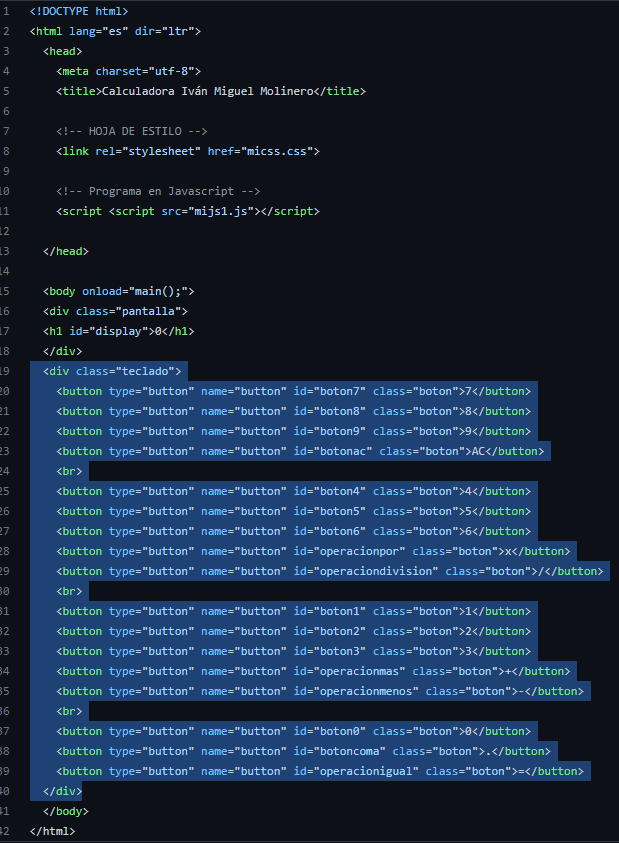
\includegraphics[width=10cm, keepaspectratio]{img/html.png}
  \caption{Fragmento HTML}\label{fig:html}
\end{figure}
\\

\section{CSS}
\label{sec:CSS}

CSS\cite{website:CSS} (del inglés Cascading Style Sheets) es utilizado para dar estilo a las páginas web creadas con HTML o XML. Ha tenido varias versiones pero es desde CSS3 que su alcance es tal que cada módulo empezó a mostrar varias diferencias por lo que el W3C\footnote{\url{https://www.w3.org/}}  decidió empezar a realizar capturas de las últimas especificaciones estables.

Su sintaxis más básica consiste en hacer referencia a las diferentes etiquetas de HTML y definir su estilo entre corchetes. Por ejemplo:

\begin{verbatim}
div {
    text-align: center;
}

img {
  height: 20px;
  margin-left: 0px;
}
\end{verbatim}

\section{Javascript}
\label{sec:Javascript}

Javascript\cite{website:Javascript} (abreviado JS) es un lenguaje de programación ligero, interpretado y compilado ``just-in-time´´. Se usa para secuencias de comandos en páginas web aunque también se utiliza en otros entornos como Node.js\footnote{\url{https://developer.mozilla.org/es/docs/Glossary/Node.js}}.

Se originó en el año 1995 para el navegador Netscape como una forma de agregar programas a páginas web. Desde entonces, el lenguaje ha sido adoptado por todos los demás navegadores gráficos principales. Ha hecho posibles las aplicaciones web modernas, aplicaciones con las que puede interactuar directamente sin hacer una recarga de página para cada acción.

Algunas de las características de Javascript son las siguientes:

\begin{itemize}
	\item Lenguaje del lado del cliente
	\item Orientado a objetos
	\item De tipado débil o no tipado
	\item De alto nivel
	\item Lenguaje interpretado
	\item Muy utilizado por los desarrolladores\\
\end{itemize}

\section{OpenBRR}
\label{sec:openbrr}

OpenBRR\cite{website:OpenBRR} (del inglés Business Readiness Rating) es un modelo de evaluación de software libre. Su objetivo es estandarizar una fórmula de evaluación de software. Este método fue patrocinado por el Centro de Investigación de Código abierto e Intel.

Se considera necesario ya que proporciona a las compañías una forma segura, estandarizada y eficaz de evaluar un software antes de adoptarlo. Hasta el momento ha permitido a compañías tanto elegir un software ideal para misiones críticas como descartar otros que a primera vista parecían buenos pero que después de analizarlos dieron con graves problemas de seguridad.

El esquema de análisis se puede ver en la siguiente figura.

\begin{figure}
  \centering
  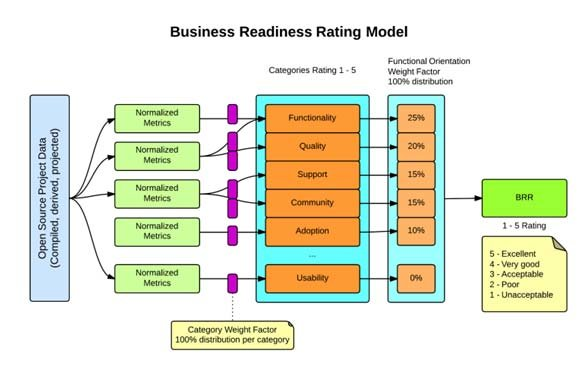
\includegraphics[width=14cm, keepaspectratio]{img/openbrr.png}
  \caption{Esquema de análisis de OpenBRR}\label{fig:OpenBRR}
\end{figure}


%%%%%%%%%%%%%%%%%%%%%%%%%%%%%%%%%%%%%%%%%%%%%%%%%%%%%%%%%%%%%%%%%%%%%%%%%%%%%%%%
%%%%%%%%%%%%%%%%%%%%%%%%%%%%%%%%%%%%%%%%%%%%%%%%%%%%%%%%%%%%%%%%%%%%%%%%%%%%%%%%
% DISEÑO E IMPLEMENTACIÓN %
%%%%%%%%%%%%%%%%%%%%%%%%%%%%%%%%%%%%%%%%%%%%%%%%%%%%%%%%%%%%%%%%%%%%%%%%%%%%%%%%

\cleardoublepage
\chapter{Diseño e implementación}

Aquí viene todo lo que has hecho tú (tecnológicamente). 
Puedes entrar hasta el detalle. 
Es la parte más importante de la memoria, porque describe lo que has hecho tú.
Eso sí, normalmente aconsejo no poner código, sino diagramas.

\section{Arquitectura general} 
\label{sec:arquitectura}

Si tu proyecto es un software, siempre es bueno poner la arquitectura (que es cómo se estructura tu programa a ``vista de pájaro'').

Por ejemplo, puedes verlo en la figura~\ref{fig:arquitectura}.
\LaTeX \ pone las figuras donde mejor cuadran. 
Y eso quiere decir que quizás no lo haga donde lo hemos puesto\ldots
Eso no es malo.
A veces queda un poco raro, pero es la filosofía de \LaTeX: tú al contenido, que yo me encargo de la maquetación.

\begin{figure}
  \centering
  \includegraphics[width=9cm, keepaspectratio]{img/arquitectura.png}
  \caption{Estructura del parser básico.}\label{fig:arquitectura}
\end{figure}

\begin{figure}
    \centering
    \includegraphics[bb=0 0 800 600, width=12cm, keepaspectratio]{img/foro1}
    \caption{Página con enlaces a hilos}\label{fig:_arquitectura}
\end{figure}

 
Recuerda que toda figura que añadas a tu memoria debe ser explicada.
Sí, aunque te parezca evidente lo que se ve en la figura~\ref{fig:arquitectura}, la figura en sí solamente es un apoyo a tu texto.
Así que explica lo que se ve en la figura, haciendo referencia a la misma tal y como ves aquí.
Por ejemplo: En la figura~\ref{fig:arquitectura} se puede ver que la estructura del \emph{parser} básico, que consta de seis componentes diferentes: los datos se obtienen de la red, y según el tipo de dato, se pasará a un \emph{parser} específico y bla, bla, bla\ldots

Si utilizas una base de datos, no te olvides de incluir también un diagrama de entidad-relación.


%%%%%%%%%%%%%%%%%%%%%%%%%%%%%%%%%%%%%%%%%%%%%%%%%%%%%%%%%%%%%%%%%%%%%%%%%%%%%%%%
%%%%%%%%%%%%%%%%%%%%%%%%%%%%%%%%%%%%%%%%%%%%%%%%%%%%%%%%%%%%%%%%%%%%%%%%%%%%%%%%
% EXPERIMENTOS Y VALIDACIÓN %
%%%%%%%%%%%%%%%%%%%%%%%%%%%%%%%%%%%%%%%%%%%%%%%%%%%%%%%%%%%%%%%%%%%%%%%%%%%%%%%%

\cleardoublepage
\chapter{Experimentos y validación}

Este capítulo se introdujo como requisito en 2019. 
Describe los experimentos y casos de test que tuviste que implementar para validar tus resultados. 
Incluye también los resultados de validación que permiten afirmar que tus resultados son correctos. 


%%%%%%%%%%%%%%%%%%%%%%%%%%%%%%%%%%%%%%%%%%%%%%%%%%%%%%%%%%%%%%%%%%%%%%%%%%%%%%%%
%%%%%%%%%%%%%%%%%%%%%%%%%%%%%%%%%%%%%%%%%%%%%%%%%%%%%%%%%%%%%%%%%%%%%%%%%%%%%%%%
% RESULTADOS %
%%%%%%%%%%%%%%%%%%%%%%%%%%%%%%%%%%%%%%%%%%%%%%%%%%%%%%%%%%%%%%%%%%%%%%%%%%%%%%%%

\cleardoublepage
\chapter{Resultados}

En este capítulo se incluyen los resultados de tu trabajo fin de grado.

Si es una herramienta de análisis lo que has realizado, aquí puedes poner ejemplos de haberla utilizado para que se vea su utilidad.


%%%%%%%%%%%%%%%%%%%%%%%%%%%%%%%%%%%%%%%%%%%%%%%%%%%%%%%%%%%%%%%%%%%%%%%%%%%%%%%%
%%%%%%%%%%%%%%%%%%%%%%%%%%%%%%%%%%%%%%%%%%%%%%%%%%%%%%%%%%%%%%%%%%%%%%%%%%%%%%%%
% CONCLUSIONES %
%%%%%%%%%%%%%%%%%%%%%%%%%%%%%%%%%%%%%%%%%%%%%%%%%%%%%%%%%%%%%%%%%%%%%%%%%%%%%%%%

\cleardoublepage
\chapter{Conclusiones}
\label{chap:conclusiones}


\section{Consecución de objetivos}
\label{sec:consecucion-objetivos}

Esta sección es la sección espejo de las dos primeras del capítulo de objetivos, donde se planteaba el objetivo general y se elaboraban los específicos.

Es aquí donde hay que debatir qué se ha conseguido y qué no. 
Cuando algo no se ha conseguido, se ha de justificar, en términos de qué problemas se han encontrado y qué medidas se han tomado para mitigar esos problemas.

Y si has llegado hasta aquí, siempre es bueno pasarle el corrector ortográfico, que las erratas quedan fatal en la memoria final.
Para eso, en Linux tenemos aspell, que se ejecuta de la siguiente manera desde la línea de \emph{shell}:

\begin{verbatim}
  aspell --lang=es_ES -c memoria.tex
\end{verbatim}

\section{Aplicación de lo aprendido}
\label{sec:aplicacion}

Aquí viene lo que has aprendido durante el Grado/Máster y que has aplicado en el TFG/TFM. Una buena idea es poner las asignaturas más relacionadas y comentar en un párrafo los conocimientos y habilidades puestos en práctica.

\begin{enumerate}
  \item a
  \item b
\end{enumerate}


\section{Lecciones aprendidas}
\label{sec:lecciones_aprendidas}

Aquí viene lo que has aprendido en el Trabajo Fin de Grado/Máster.

\begin{enumerate}
  \item Aquí viene uno.
  \item Aquí viene otro.
\end{enumerate}


\section{Trabajos futuros}
\label{sec:trabajos_futuros}

Ningún proyecto ni software se termina, así que aquí vienen ideas y funcionalidades que estaría bien tener implementadas en el futuro.

Es un apartado que sirve para dar ideas de cara a futuros TFGs/TFMs.


%%%%%%%%%%%%%%%%%%%%%%%%%%%%%%%%%%%%%%%%%%%%%%%%%%%%%%%%%%%%%%%%%%%%%%%%%%%%%%%%
%%%%%%%%%%%%%%%%%%%%%%%%%%%%%%%%%%%%%%%%%%%%%%%%%%%%%%%%%%%%%%%%%%%%%%%%%%%%%%%%
% APÉNDICE(S) %
%%%%%%%%%%%%%%%%%%%%%%%%%%%%%%%%%%%%%%%%%%%%%%%%%%%%%%%%%%%%%%%%%%%%%%%%%%%%%%%%

\cleardoublepage
\appendix
\chapter{Manual de usuario}
\label{app:manual}

Esto es un apéndice.
Si has creado una aplicación, siempre viene bien tener un manual de usuario.
Pues ponlo aquí.

%%%%%%%%%%%%%%%%%%%%%%%%%%%%%%%%%%%%%%%%%%%%%%%%%%%%%%%%%%%%%%%%%%%%%%%%%%%%%%%%
%%%%%%%%%%%%%%%%%%%%%%%%%%%%%%%%%%%%%%%%%%%%%%%%%%%%%%%%%%%%%%%%%%%%%%%%%%%%%%%%
% BIBLIOGRAFIA %
%%%%%%%%%%%%%%%%%%%%%%%%%%%%%%%%%%%%%%%%%%%%%%%%%%%%%%%%%%%%%%%%%%%%%%%%%%%%%%%%

\cleardoublepage

% Las siguientes dos instrucciones es todo lo que necesitas
% para incluir las citas en la memoria
\bibliographystyle{abbrv}
\bibliography{memoria}  % memoria.bib es el nombre del fichero que contiene
% las referencias bibliográficas. Abre ese fichero y mira el formato que tiene,
% que se conoce como BibTeX. Hay muchos sitios que exportan referencias en
% formato BibTeX. Prueba a buscar en http://scholar.google.com por referencias
% y verás que lo puedes hacer de manera sencilla.
% Más información: 
% http://texblog.org/2014/04/22/using-google-scholar-to-download-bibtex-citations/

\end{document}
